% \documentclass[preprint,12pt]{elsarticle}
\documentclass[preprint,1p,12pt,authoryear]{elsarticle} % EAAI
\usepackage[x11names]{xcolor}
\usepackage{fontawesome5}
\usepackage{amssymb}
\usepackage{url}
\usepackage{amsmath}
\usepackage{hyperref} 

\usepackage[utf8]{inputenc}
\usepackage{amsfonts}
\usepackage{booktabs}
\usepackage{nicefrac}
\usepackage{multirow}
\usepackage{geometry}
\usepackage{setspace}
\usepackage{url}
\usepackage{hyperref}
\usepackage{wrapfig}
% Graphics / floats
\usepackage{graphicx}
\usepackage{subcaption}
\usepackage{wrapfig}
\usepackage{forest}
\usepackage{tikz}                  
\usepackage[x11names]{xcolor}

% Algorithms / misc.
\usepackage{algorithm}
\usepackage{algpseudocode}
\usepackage{marvosym}
\usepackage{color}
\usepackage{mathrsfs}

\usepackage{booktabs}
\usepackage{siunitx}
\usepackage{multirow} % 
\usepackage{makecell} % 
% ----------------------------------------------------------------
% Custom colours & TikZ / forest styles
% ----------------------------------------------------------------
\definecolor{hidden-draw}{RGB}{255,255,255}
\definecolor{hidden-pink}{RGB}{255,182,193}
\definecolor{level0}{RGB}{240,248,255}
\definecolor{level1}{RGB}{224,240,255}
\definecolor{darkgray}{gray}{0.30}

\tikzstyle{my-box}=[
    rectangle,
    draw=hidden-draw,
    rounded corners,
    text opacity=1,
    minimum height=1.5em,
    minimum width=5em,
    inner sep=2pt,
    align=center,
    fill opacity=.5,
    line width=0.8pt,
]
\tikzstyle{leaf}=[
    my-box,
    minimum height=1.5em,
    fill=hidden-pink!80,
    text=black,
    align=left,
    font=\normalsize,
    inner xsep=2pt,
    inner ysep=4pt,
    line width=0.8pt,
]

\usepackage{amsthm} 
\newtheorem{assumption}{Assumption} 
\usepackage{filecontents}
\usepackage{threeparttable}
\usepackage{siunitx}
\usepackage{soul} 
\usepackage{tabularx}
\usepackage{array}
\usepackage{ragged2e}
\usepackage{tcolorbox}
\usepackage[utf8]{inputenc}
\usepackage{hyperref}



\newif\ifblind
\blindtrue   % EAAI
% \blindfalse

\journal{Integrating Large Language Models into Portfolio Optimization: A Black-Litterman Approach} % EAAI

\begin{document}
\begin{frontmatter}


% \title{LLM-Enhanced Black-Litterman Portfolio Optimization}
\title{Integrating Large Language Models into Portfolio Optimization: A Black-Litterman Approach} % EAAI
% -----------------------------------------------------------
% [수정된 부분] 스위치에 따라 저자 정보를 숨기거나 표시합니다
% -----------------------------------------------------------
\ifblind
    % === Blind Mode (심사용) ===
    % 저자 정보가 완전히 숨겨집니다.
    % 필요하다면 아래 주석을 풀어 "Anonymous Authors"라고 표시할 수도 있습니다.
    \author{Anonymous Authors}
\else
    % === Non-Blind Mode (최종본/아카이브용) ===
    %% --- First Line Authors ---
    \author[inst1]{Youngbin Lee\fnref{equal}}
    \author[inst2]{Yejin Kim\fnref{equal}}
    \author[inst3]{Juhyeong Kim}
    \author[inst1]{Suin Kim}
    
    %% --- Second Line Authors ---
    \author[inst4]{Yoontae Hwang\corref{cor1}}
    \ead{yoontae.hwang@pusan.ac.kr}
    \author[inst5]{Yongjae Lee\corref{cor1}}
    \ead{yongjaelee@unist.ac.kr}
    
    %% Footnotes
    \fntext[equal]{Equal contribution}
    \cortext[cor1]{Corresponding authors.}
    
    %% Affiliations
    \affiliation[inst1]{organization={Elice},
                city={Seoul},
                country={Republic of Korea}}
    
    \affiliation[inst2]{organization={Meritz Fire \& Marine Insurance},
                city={Seoul},
                country={Republic of Korea}}
    
    \affiliation[inst3]{organization={Mirae Asset Global Investments},
                city={Seoul},
                country={Republic of Korea}}
    
    \affiliation[inst4]{organization={Pusan National University},
                city={Busan},
                country={Republic of Korea}}
    
    \affiliation[inst5]{organization={Ulsan National Institute of Science and Technology},
                city={Ulsan},
                country={Republic of Korea}}
\fi
% -----------------------------------------------------------


\begin{abstract}
Large language models (LLMs) have demonstrated remarkable capabilities in analyzing financial text and generating market insights. However, integrating these unstructured and often qualitative outputs into disciplined quantitative portfolio construction remains a challenge. To bridge this gap, this study proposes a systematic framework that operationalizes LLM capabilities within the Black-Litterman model. Instead of relying on single-point estimates, we treat LLM-generated forecasts as probabilistic distributions. We map the mean of stochastic draws to investor views and their dispersion to view confidence levels.  This approach provides an auditable route to incorporate LLM-driven signals into rigorous mean-variance optimization. We validated this methodology through an out-of-sample backtest on a universe of large-cap U.S. equities. The results indicate that portfolios driven by propsed framework showed favorable risk-adjusted returns compared to equal-weight and traditional mean-variance benchmarks. These findings demonstrate that our framework effectively translates the predictive power of LLMs into systematic asset allocation.
The source code and data are available at: \faGithub \href{https://anonymous.4open.science/r/FRL2026-E3E5}{LLM-BLM} 
\end{abstract}

\begin{highlights} % EAAI: 공백 포함 85자 이내! (Highlights should consist of 3 to 5 bullet points, each a maximum of 85 characters, including spaces.)
\item A systematic framework integrating large language models into Black-Litterman model.
\item Maps AI forecast distributions to investor views and confidence levels.
\item Provides an auditable pipeline for AI-driven quantitative asset allocation.
\end{highlights}

%% Keywords
\begin{keyword} 
Black-Litterman model
\sep Large Language Models
\sep Portfolio optimization


\end{keyword}

\end{frontmatter}




% \newpage
% \thispagestyle{empty} % Title page에는 페이지 번호 제거

% \begin{center}
%     \vspace*{2cm}

%     % 1. Title
%     % {\Large \textbf{LLM-Enhanced Black-Litterman Portfolio Optimization}}
%     {\Large \textbf{Enhancing Black-Litterman Portfolio Optimization with Large Language Models}} % EAAI에서는 제목에 약어 사용 금지
%     \vspace{2cm}

%     % 2. Author Names
%     {\large
%         Youngbin Lee\textsuperscript{a,1},
%         Yejin Kim\textsuperscript{b,1},
%         Juhyeong Kim\textsuperscript{c},
%         Suin Kim\textsuperscript{a}, \\[5pt]
%         Yoontae Hwang\textsuperscript{d,*} and
%         Yongjae Lee\textsuperscript{e,*}
%     }

%     \vspace{1.5cm}

%     % 3. Affiliations
%     {\normalsize
%         \textsuperscript{a}Elice, Seoul, Republic of Korea \\
%         \textsuperscript{b}Meritz Fire \& Marine Insurance, Seoul, Republic of Korea \\
%         \textsuperscript{c}Mirae Asset Global Investments, Seoul, Republic of Korea \\
%         \textsuperscript{d}Pusan National University, Busan, Republic of Korea \\
%         \textsuperscript{e}Ulsan National Institute of Science and Technology, Ulsan, Republic of Korea
%     }

%     \vspace{3cm}

%     % 4. Contact Info / Footnotes
%     \begin{flushleft}
%         \rule{5cm}{0.5pt} \\[5pt] % 구분선
%         \footnotesize
%         \textsuperscript{1}Equal contribution. \\
%         \textsuperscript{*}Corresponding authors. \\
%         \textit{E-mail addresses:} \texttt{yoontae.hwang@pusan.ac.kr} (Yoontae Hwang), \texttt{yongjaelee@unist.ac.kr} (Yongjae Lee)
%     \end{flushleft}

% \end{center}
% \newpage


\section{Introduction}
LLMs achieve strong performance on a broad set of language tasks, and they can convert large volumes of text into structured summaries and judgments. Finance is a natural setting for these tools because much information arrives in text. News, regulatory filings, and earnings calls shape expectations long before they appear in prices. Recent studies show that language model outputs can capture signals from analyst reports \citep{kim2023llms} or financial news headlines \citep{lopez2023can}, guide asset allocation based on macroeconomic conditions \citep{kim2023if}, and uncover latent thematic structures \citep{lee2025theme}. These results point to a practical opportunity. A model that reads text can form qualitative views about the market and about individual firms, but portfolio management requires these views to influence concrete trading decisions. A practical allocator still faces a missing step. Portfolio optimization requires quantitative inputs, and it also requires uncertainty estimates so that unreliable signals do not dominate the allocation. LLMs can generate qualitative views about market sentiment and firm prospects, but there is no established systematic method that turns these unstructured insights into disciplined inputs for portfolio construction. Many existing uses of LLMs in finance stop at sentiment scores, rankings, or simple trading rules. These outputs can support analysis, but they do not provide an auditable route from language based judgments to the objects a portfolio optimizer must consume.

We fill this gap by using the Black-Litterman model as an interface between LLM generated views and quantitative allocation. Mean-variance optimization (MVO) is sensitive to error in expected returns and it can produce unstable weights when forecasts are noisy \citep{best1991sensitivity, merton1980estimating, chung2022effects}. The Black-Litterman framework mitigates this sensitivity by combining an equilibrium prior with explicit views, and by weighting each view by its stated uncertainty \citep{black1992global}. This is the structure needed to incorporate language based judgments into a standard optimization pipeline. We do not modify the Black Litterman update. We use it because it provides a clean mechanism to inject views into portfolio choice, provided we can supply view values and view uncertainty in a principled way.

We propose a data-driven mapping from LLM outputs to the inputs required by the Black-Litterman update. We treat an LLM as a stochastic return forecaster. We query the model repeatedly for the same asset and horizon under a fixed prompt and a strictly time stamped information set. This produces a distribution of numerical forecasts. We set the view to the average forecast, and we set view uncertainty to the dispersion of the forecasts. The Black-Litterman update then assigns less influence to views with high dispersion and more influence to views with low dispersion. We interpret dispersion as model uncertainty about the view rather than sampling error of the average forecast, so uncertainty does not shrink with the number of queries.

This approach operationalizes LLM capabilities for portfolio optimization without adding new modeling assumptions inside the allocator. By deriving both return forecasts and confidence levels directly from observable model outputs, the proposed method ensures an auditable route from text to portfolio weights. The approach is inherently scalable because the same procedure applies across different assets and LLMs. It also supports evaluation that matches financial practice because strict information sets prevent look-ahead contamination. In our out-of-sample backtest on a large-cap equity universe, portfolios that use this mapping within the Black-Litterman framework improve risk-adjusted performance relative to equal weight and standard mean-variance baselines after accounting for transaction costs.

%Mean–variance optimization (MVO) provides a canonical normative framework for portfolio choice, but it is fragile in practice. Small errors in expected returns generate extreme and unstable weights, undermining implementability \citep{best1991sensitivity, merton1980estimating, chung2022effects}. The Black–Litterman (BLM) model addresses this instability by combining a market‑equilibrium prior with investor views, recentering mean estimates and regularizing portfolios \citep{black1992global}. In BLM, the influence of a view depends on its level $\mathbf{q}$ and its confidence matrix $\mathbf{\Omega}$. Views with lower uncertainty receive more weight. Accordingly, the key practical question is how to specify and calibrate views and their confidence. Specifying and calibrating views has been the practical bottleneck. Standard implementations set $\mathbf{q}$ by subjective judgment and map confidence to $\mathbf{\Omega}$ using ad hoc rules \citep{he2002intuition, idzorek2007step}, choices that are hard to audit, difficult to scale, and susceptible to behavioral biases. Meanwhile, large language models (LLMs) extract forward‑looking signals from unstructured text—news, filings, and earnings calls—\citep{lopez2023can, kim2023if}. However, applications often stop at sentiment scoring or simple long–short sorts, without entering portfolio construction. The literature lacks an econometrically grounded mapping from noisy LLM predictions to the $\mathbf{q}$ and $\mathbf{\Omega}$ required by BLM. We bridge this gap with a parsimonious mapping that allows the forecasting model to quantify its own uncertainty. For each asset and forecast horizon, we query an LLM $N$ times with a fixed prompt and record $N$ stochastic draws. We set $q_i$ to the mean of the draws and set confidence to their dispersion—$\Omega_{ii}$ equals the variance for absolute views, and $\mathbf{\Omega}$ equals the full covariance matrix for joint views. The LLM’s predictive dispersion determines view confidence: high variance is automatically down‑weighted in the BLM update, whereas low variance receives greater weight. Importantly, we treat $\mathbf{\Omega}$ as model uncertainty rather than sampling error of the mean. Therefore we do not divide by $N$. This mean–variance mapping replaces subjective confidence inputs with a transparent, data‑driven procedure that scales across assets, models, and time.
\section{Related work}

\subsection{Portfolio Optimization and View Uncertainty}
Portfolio choice is difficult because the inputs are noisy, not because the optimization problem is hard \citep{markowitz1952portfolio}. The optimizer amplifies input error. Small errors in expected returns can produce large and unstable weights \citep{jobson1980estimation, best1991sensitivity}. Noise in expected returns often dominates performance out of sample, and even modest misspecification can lead to unintuitive allocations and unstable tail risk exposures \citep{merton1980estimating, chopra1993effect}. Two research lines address these issues. One line shrinks inputs through Bayes Stein mean shrinkage \citep{jorion1986bayes}, high dimensional covariance estimators \citep{ledoit2003improved, ledoit2004well}, and Bayesian priors \citep{avramov2002stock, pastor2000portfolio}. Another line regularizes the optimizer through resampling \citep{michaud1989markowitz} and robust formulations that account for model misspecification \citep{garlappi2007portfolio, bertsimas2011theory}. Many studies conclude that without strong prior structure or disciplined shrinkage, plug in mean variance optimization can underperform a simple equal weight rule \citep{demiguel2009optimal}.

Black and Litterman provide a Bayesian approach that combines an equilibrium prior with investor views \citep{black1992global}. The model uses a view uncertainty matrix to determine how strongly each view influences the posterior. This structure makes the framework well suited as an interface for external forecasts, including forecasts produced from text based models. The practical difficulty is that most applications still rely on subjective choices for both the view values and their uncertainty. Prior work explains how to express absolute and relative views \citep{he2002intuition}, and later papers clarify and extend the framework \citep{satchell2007demystification, ccela2021mean}. Industry practice often maps user reported confidence into the view uncertainty matrix through heuristic scaling rules \citep{idzorek2007step}. These choices are hard to audit, brittle across assets and horizons, and difficult to scale.

This gap matters more when views come from LLMs, since the views originate from unstructured information and the uncertainty is not directly observed. Our work follows the same goal as the prior literature on disciplined inputs, but we target the specific interface needed for optimizer level use. We elicit a forecast distribution from an LLM by repeating the same query many times under a fixed prompt, and we interpret the dispersion of the forecasts as model uncertainty about the view. We set the view to the average forecast and set view uncertainty to the forecast variance, or the forecast covariance when we elicit joint views. We treat this uncertainty as model uncertainty rather than sampling error of the average, so it does not shrink with the number of repeated queries. This mapping replaces ad hoc tuning with an auditable procedure that scales across assets, horizons, and forecasting models.

\subsection{The Missing Optimizer Link}
A parallel literature in asset pricing and corporate finance extracts forward looking information from unstructured text. Early studies show that media tone and disclosure language predict investor reactions and returns \citep{tetlock2007giving, tetlock2008more, loughran2011liability}. Surveys document the maturation of text as data, from dictionaries to machine learning and embeddings \citep{gentzkow2019text, hwang2025deep}. Large language models extend this toolkit. They can synthesize news, filings, and earnings call dialogue into forecasts at scale, and recent evidence links LLM based assessments to fundamentals and returns \citep{lopez2023can, liu2023fingpt, lee2025your}.

Two frictions keep this literature separate from formal allocation. First, most applications remain task level rather than optimizer level. Researchers often report point scores or rankings, but a portfolio optimizer needs a clear view value and a defensible measure of view uncertainty. When portfolios are formed, signal strength is usually implicit, so the optimizer cannot control exposure to uncertain views. Second, evaluation practices often fall short of financial econometric standards. General purpose LLMs are trained on corpora that include financial text, so backtests without verified knowledge cutoffs and strict time stamping risk look ahead and data contamination. This compounds classic concerns about multiple testing and data snooping \citep{bender2021dangers, drinkall2024time, kong2025fusing}.

Our work connects these threads by providing a concrete mapping from LLM outputs to the inputs required by a Bayesian optimizer. We treat the LLM forecast average as the view and the forecast dispersion as view uncertainty, and we enforce strict knowledge cutoffs and time stamped information sets to prevent contamination. This design allows language based forecasts to enter portfolio optimization on disciplined terms and enables direct evaluation of how uncertainty calibration affects allocation outcomes.


\section{Methodology} \label{sec:method}
We estimate view vector and view confidence matrix, $(\mathbf{q}_t,\mathbf{\Omega}_t)$, from an LLM’s predictive distribution for $h$‑day ahead excess returns. For each asset and decision time $t$, we elicit $N$ stochastic forecasts under a fixed prompt and model state and set $q_{i,t}$ to the sample mean of the draws, while $\Omega_{ii,t}$ equals their sample variance. We interpret $\mathbf{\Omega}_t$ as model uncertainty about the view, not sampling error of $\hat{\mathbf{q}}_t$, so we do not divide by $N$. This mapping replaces subjective confidence inputs with an auditable, data‑driven rule in which higher predictive dispersion automatically down‑weights a view in the Black-Litterman update. Figure \ref{fig:model} summarizes the workflow.

\begin{figure*}[h!]
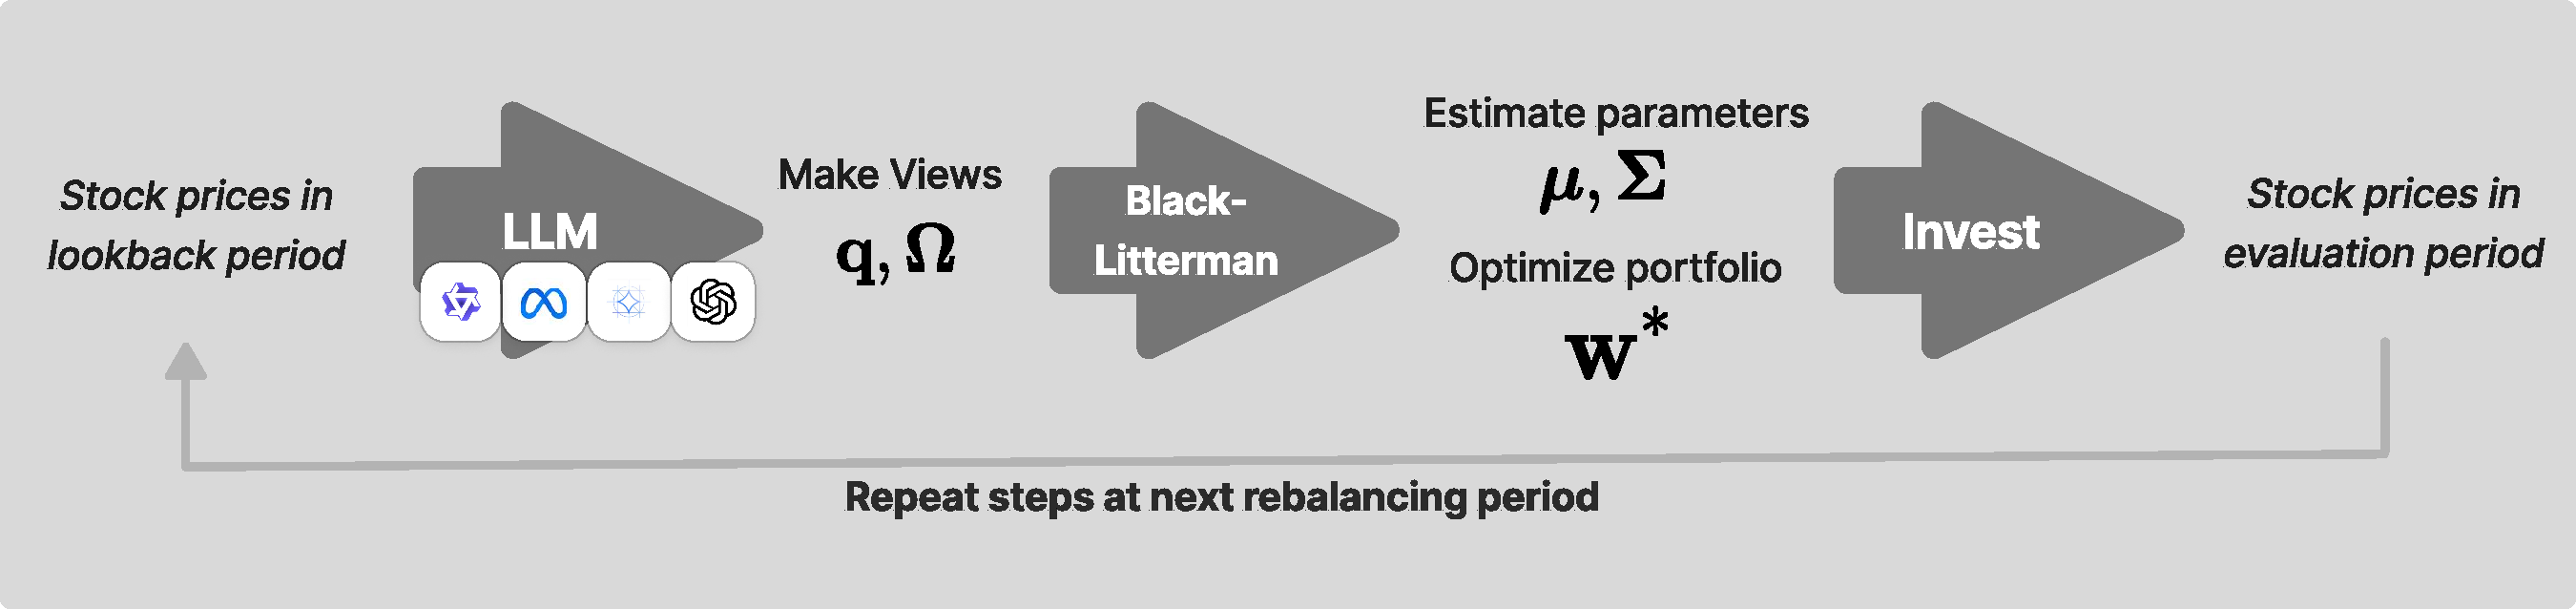
\includegraphics[width=1\linewidth]{figure/model.pdf}
\caption{\textbf{Workflow for mapping LLM predictive distributions into Black-Litterman views.} At decision time $t$, $N$ stochastic LLM forecasts of $h$‑day excess returns yield $\mathbf{q}_t$ and $\mathbf{\Omega}_t$, which combine with the equilibrium prior to form posterior expected returns used for portfolio optimization.}
\label{fig:model}
\end{figure*}

\subsection{A Framework for Prompt‑based Black–Litterman Views}
\textbf{Setup} Fix a decision time $t$ and $n$ assets. Let $h$ denote the forecast horizon, and let $\mathbf{r}_{t:t+h}\in\mathbb{R}^n$ be the vector of $h$‑day excess returns. Under a fixed prompt $\mathcal{P}$ and a fixed model state $\mathcal{S}_t$, the LLM acts as a stochastic forecast generator. For each asset $i$, the model induces a predictive distribution
\begin{equation}
    \tilde{Q}_{i, t} \sim F_{i, t}\left(\cdot \mid \mathcal{P}, \mathcal{S}_t\right)
\end{equation}
where a query samples $\tilde{Q}_{i,t}$ via internal randomness. We issue $N$ queries with $(\mathcal{P},\mathcal{S}_t)$ held fixed and obtain draws $\{\tilde{q}^{(j)}_{i,t}\}_{j=1}^N$. To elicit quantitative views, we use a two‑part prompt. The system prompt instructs the model to output a single scalar representing the $h$‑day expected excess return (in decimals) for a specified ticker, under a fixed output schema that rejects non‑numeric text. The user prompt provides only information timestamped $\le t$: (i) the asset’s recent return series, (ii) sector and market benchmark returns over the same window, and (iii) static metadata (ticker, name, GICS sector/sub‑industry). Section~\ref{appendix:prompts} lists the exact prompts and schema.

\textbf{Estimators} For asset $i$ at time $t$, let
\begin{equation}
    \hat{q}_{i, t}=\frac{1}{N} \sum_{j=1}^N \tilde{q}_{i, t}^{(j)}, \quad \hat{\sigma}_{i, t}^2=\frac{1}{N-1} \sum_{j=1}^N\left(\tilde{q}_{i, t}^{(j)}-\hat{q}_{i, t}\right)^2.
\end{equation}
We interpret $\hat{\sigma}^2_{i,t}$ as the variance of the predictive distribution, not the variance of the sample mean, so it is not divided by $N$. In implementation we apply a small variance floor $\varepsilon>0$ to avoid numerical singularity.



\textbf{Assembling views} We aggregate the individual estimates into the view vector $\mathbf{q}_t=(\hat{q}_{1,t},\ldots,\hat{q}_{n,t})'$ and the diagonal covariance matrix $\mathbf{\Omega}_t=\mathrm{diag}(\hat{\sigma}^2_{1,t},\ldots,\hat{\sigma}^2_{n,t})$. 
Because we generate forecasts asset‑by‑asset, $\mathbf{\Omega}_t$ is diagonal. So, a joint‑view extension would estimate the full covariance from simultaneous multi‑asset draws.
To utilize these inputs in the Black–Litterman framework, we must also specify the picking matrix $\mathbf{P}$, which maps each view to the underlying assets in the portfolio. Since our methodology generates a direct absolute return forecast for every asset in the universe (1-to-1 mapping), we define $\mathbf{P}$ as the $n \times n$ identity matrix ($\mathbf{P}=\mathbf{I}_n$).
This structure implies that the $i$-th view corresponds exclusively to the $i$-th asset (i.e., $P_{ii}=1$ and $P_{ij}=0$ for $i \neq j$), treating each forecast as an absolute view.
Consequently, the estimation provides a complete set of inputs $(\mathbf{q}_t, \mathbf{\Omega}_t, \mathbf{P})$ required for the posterior update in Equation (\ref{eq:BlackLitterman}).

\subsection{Prompt Design Details} \label{appendix:prompts}

To clarify the temporal context for the return prediction task, we include an explicit reference date in the system prompt (Figure~\ref{fig:system_prompt}). This date represents the point in time at which the LLM is expected to provide its analysis—positioned between the past time series data and the future return period. By anchoring the prediction task to a specific date, we help the model better interpret the directionality of the input data and generate temporally coherent forecasts.

To ensure consistent and parseable responses from the LLMs, we adopt a structured output format using the JSON schema supported by the chat completions API endpoint. This approach standardizes the outputs across all LLMs and ensures that each model provides consistently structured responses across repeated queries, reducing the likelihood of formatting errors and facilitating reliable downstream processing.

To enhance the models' numerical sensitivity, all daily return inputs are scaled by 100 (i.e., presented in percentage terms) in the user prompt (Figure~\ref{fig:user_prompt}). For instance, a daily return of -0.0036 is provided as -0.36. This scaling prevents issues arising from the small magnitude of raw daily returns, which can be difficult for LLMs to differentiate and process effectively. This approach is analogous to using basis points in finance to handle small numerical values. By providing a rich, multi-faceted data context and clear instructions, the prompts enable the LLMs to generate informed, quantitative views for portfolio construction.

\begin{figure}[htbp]
\centering
    \scalebox{0.92}{%
    \begin{tcolorbox}[colframe=blue!80!black, colback=blue!10!white, coltitle=white, title=System Prompt, width=1.08\columnwidth]
    \scriptsize
    \setlength{\itemsep}{1pt}%
    \setlength{\topsep}{2pt}%
    \setlength{\partopsep}{0pt}%
    \setlength{\parsep}{0pt}%
    You are providing analysis on \texttt{{\{\{DATE\}\}}}. Predict the average daily return for the next two weeks based on the information provided about a stock's past performance.
    You will receive the following inputs:
    \begin{itemize}
        \item \textbf{Daily Returns}: The stock's daily returns, a time-series from the past two weeks.
        \item \textbf{Company Sector}: The company's GICS sector classification.
        \item \textbf{Sector Returns}: The company sector's daily returns, a time-series from the past two weeks.
        \item \textbf{Market Returns}: The S\&P 500's daily returns, a time-series from the past two weeks.
        \item \textbf{Company Information}:
            \begin{itemize}
                \item Ticker: The stock symbol.
                \item Company Name: The name of the company.
                \item GICS Sector: The Global Industry Classification Standard sector.
                \item GICS Sub-Industry: The sub-industry classification.
            \end{itemize}
    \end{itemize}
    
    \# Steps
    \begin{enumerate}
        \item \textbf{Analyze the Time-Series Data}: Review the historical daily returns to identify patterns, trends, or anomalies that may affect future performance.
        \item \textbf{Consider Sector Performance}: Analyze how the market and the sector's performance might influence the stock's future returns.
        \item \textbf{Incorporate Company Information}: Use the details from the GICS sector and sub-industry, along with the company symbol and name, to contextualize the predicted performance within its industry.
        \item \textbf{Predict Future Returns}: Estimate the average daily returns for the next two weeks based on the analysis of available data.
    \end{enumerate}
    
    \# Output Format
    \begin{quote}
    Return a single float value that represents the predicted average daily return for the stock over the next two weeks, without any additional commentary or explanation.
    \end{quote}
    
    \# Notes
    \begin{itemize}
        \item Ensure the prediction considers the quantified data from the time-series.
        \item Make calculations based on statistical trends from daily returns data.
        \item Pay attention to the trends within both the stock's daily returns and the market's return data.
        \item Consider the relevance of the company's sector to refine your predictions.
        \item Make calculations without additional interpretation or commentary.
    \end{itemize}
    
    \end{tcolorbox}%
    }
    \caption{The structure of the system prompt used to elicit return forecasts from the LLMs.}
    \label{fig:system_prompt}
\end{figure}



 % \label{fig:system_prompt}

\begin{figure}[htbp]
\centering
    \scalebox{0.92}{%
    \begin{tcolorbox}[colframe=green!60!black, colback=green!5!white, coltitle=white, title=User Prompt, width=1.08\columnwidth]
    \scriptsize
    \ttfamily % Use a typewriter font for code-like text
    \textbf{Daily Returns:} [-1.17, -0.92, -2.31, -0.36, -3.02, 2.53, 0.1, -0.23, 0.45]
    
    \vspace{0.5mm}
    \textbf{Company Sector:} Information Technology
    
    \vspace{0.5mm}
    \textbf{Sector Returns:} [-0.14, -0.38, -1.88, 0.03, -1.1, 2.38, -0.41, 0.17, -0.31]
    
    \vspace{0.5mm}
    \textbf{Market Returns:} [0.09, -0.39, -1.61, -0.04, -0.67, 2.05, -0.56, 0.4, -0.01]
    
    \vspace{0.5mm}
    \textbf{Company Information:}
    
    \hspace{5mm} \textbf{Ticker:} AAPL
    
    \hspace{5mm} \textbf{Company Name:} Apple Inc.
    
    \hspace{5mm} \textbf{GICS sector:} Information Technology
    
    \hspace{5mm}     \textbf{GICS sub-industry:} Technology Hardware, Storage \& Peripherals
    
    \end{tcolorbox}%
    }
    \caption{An example user prompt providing data for Apple Inc. (AAPL) on a specific rebalancing date.}
    \label{fig:user_prompt}
\end{figure} % \label{fig:user_prompt}

\subsection{Integrating LLM views into the Black–Litterman model} 
Let $\boldsymbol{\Pi}_t=\delta_t\,\boldsymbol{\Sigma}_t\,\mathbf{w}_{m,t}$ denote the equilibrium $h$-day excess returns implied by the market portfolio $\mathbf{w}_{m,t}$, where $\delta_t>0$ is the representative risk‑aversion scalar, $\boldsymbol{\Sigma}_t$ is the $h$‑day covariance of excess returns estimated from a trailing window, and $m$ indexes the $m$-th asset out of a total of $n$ assets ($m=1,\ldots,n$). Let $\tau>0$ scale prior uncertainty. For picking matrix $\mathbf{P}$, views $\mathbf{q}_t$, and view confidence $\mathbf{\Omega}_t$, the posterior mean of the Black–Litterman model (BLM) is
\begin{equation} \label{eq:BlackLitterman}
    \boldsymbol{\mu}_{\text{BLM}, t}=\left[\left(\tau \boldsymbol{\Sigma}_t\right)^{-1}+\mathbf{P}^{\top} \boldsymbol{\Omega}_t^{-1} \mathbf{P}\right]^{-1}\left[\left(\tau \boldsymbol{\Sigma}_t\right)^{-1} \mathbf{\Pi}_t+\mathbf{P}^{\top} \boldsymbol{\Omega}_t^{-1} \mathbf{q}_t\right].
\end{equation}

We estimate $\delta_t$ as the market price of risk at the $h$-day horizon—computed over the same window as $\boldsymbol{\Sigma}_t$. That is, 
\begin{equation}
    \delta_t = \frac{\widehat{\mathbb{E}}\left[r_{m,t:t+h}^{\text{ex}}\right]}{\widehat{\mathrm{Var}}\left(r_{m,t:t+h}^{\text{ex}}\right)}
\end{equation}
We treat $\tau$ as an ex‑ante hyperparameter and apply standard regularization to ensure numerical stability.
%We calibrate $\delta_t$ by matching the market Sharpe ratio over the estimation window and treat $\tau$ as an ex‑ante hyperparameter. Matrices are regularized to ensure numerical invertibility.

We implement a fixed‑interval rebalancing scheme with horizon $h$. At each decision time $t$: (i) we construct the information set using a rolling lookback window, (ii) elicit $N$ stochastic LLM forecasts to form $(\mathbf{q}_t,\mathbf{\Omega}_t)$, (iii) compute $\boldsymbol{\Pi}_t$ and $\boldsymbol{\Sigma}_t$ at the same horizon $h$, (iv) obtain $\boldsymbol{\mu}_{\text{BLM},t}$ from the BLM update, and (v) solve a mean–variance program
\begin{equation}
    \min _{\mathbf{w}} \lambda \mathbf{w}^{\top} \boldsymbol{\Sigma}_t \mathbf{w} - \mathbf{w}^{\top} \boldsymbol{\mu}_{\text{BLM}, t} \quad \text { s.t. } \quad \mathbf{1}^{\top} \mathbf{w}=1, \mathbf{w} \in \mathcal{C},
\end{equation}
where $\lambda$ is risk aversion and $\mathcal{C}$ encodes portfolio constraints. We hold $\mathbf{w}_t$ for $h$ days and repeat.
\section{Experiment}

This section describes the dataset, the prompting and sampling procedure used to generate LLM views, and the backtest protocol used to evaluate the BLM portfolios.

\subsection{Data Description}

We analyze daily adjusted prices from Yahoo Finance for a universe of the 50 largest S\&P 500 constituents as of March 26, 2025. The sample spans from June 2024 to June 2025. Simple daily returns are aggregated to $h$-day excess returns to match the rebalancing horizon. Note that because the universe is defined based on end‑of‑sample size ranks, results are conditional on this fixed universe and may reflect survivorship bias. 

We divide the sample into two non‑overlapping periods:
\begin{itemize}
    \item \textbf{Validation (June 1, 2024 -- August 31, 2024):} This 3-month period is used exclusively to tune the BLM hyperparameter $\tau$.
    \item \textbf{Test (September 1, 2024 -- June 30, 2025):} This 10-month period is reserved for out-of-sample evaluation. All model choices and parameters are fixed prior to this period.
\end{itemize}

We rebalance every ($h$=10) trading days. At each decision date $t$ (close), the LLM receives only information timestamped $\le$ $t$: the last $h$ trading days of prices and benchmark returns, plus static metadata (ticker, name, GICS sector/sub‑industry). The resulting views target the next $h$ trading days $[t+1, t+h]$. Portfolios are formed at $t+1$ open and held through $t+h$.
To quantify uncertainty, we perform $N=100$ independent inference runs per asset at each step. The resulting distribution of forecasts targets returns for the subsequent window $[t+1, t+h]$. Portfolios are formed at the open of $t+1$ and held until $t+h$.

\subsection{LLM Selection and Inference Protocol}

We elicit quantitative asset‑level forecasts from instruction‑tuned LLMs using a fixed schema prompt. 
To guarantee the validity of our out-of-sample evaluation, we selected models with training cutoffs pre-dating June 2024, which is well before the start of our backtesting. Table~\ref{tab:llm_summary} lists the specific versions, parameter sizes, release dates, and developers.

Inference uses vLLM \citep{kwon2023efficient} with fixed decoding settings to generate $N$ stochastic draws per asset per date.
The sample mean and variance form $(q_{i,t}, \Omega_{ii,t})$ as described in Section~\ref{sec:method}.
We employ the default sampling temperature of $T=1.0$. This choice is deliberate: rather than artificially collapsing the distribution via low-temperature greedy sampling, we aim to capture the model's intrinsic epistemic uncertainty. By sampling directly from the unscaled logit distribution, the resulting variance among the $N$ draws serves as a faithful proxy for the model's confidence ($\Omega$) in its view.

\begin{table}[h]
    \centering
    \begin{threeparttable}
        \caption{\textbf{Summary of LLMs used in this study.}}
        \label{tab:llm_summary}

        \small 
        
        \renewcommand{\arraystretch}{1.2}
        \begin{tabular}{llll}
            \hline
            \textbf{Model} & \textbf{Size} & \textbf{Release} & \textbf{Developer} \\
            \hline
            \textbf{\texttt{Gemma-7B}} \cite{team2024gemma}       & 7B      & Feb 2024 & Google DeepMind \\
            \textbf{\texttt{Qwen-2-7B}} \cite{yang2024qwen2technicalreport}    & 7B      & Jun 2024 & Alibaba Cloud \\
            \textbf{\texttt{Llama-3.1-8B}} \cite{dubey2024llama}   & 8B      & Jul 2024 & Meta \\
            \textbf{\texttt{GPT-4o-mini}} \cite{openai2024gpt4o}    & 8B \tnote{a} & Jul 2024 & OpenAI \\
            \hline
        \end{tabular}
        \begin{tablenotes}
            \scriptsize
            \item[a] Although the exact size of \texttt{GPT-4o-mini} has not been officially disclosed, \cite{abacha2024medec} estimate it to be within the 8 billion parameter range, making it comparable to the open-source models used in our study.
        \end{tablenotes}
    \end{threeparttable}
\end{table}














\section{Analysis}

We conduct an empirical backtest to evaluate the performance of our proposed framework, which integrates LLM-generated views into the BLM. To structure our analysis, we address the following key research questions:

\begin{itemize}
    \item[\textbf{RQ1}] \textit{(Performance \& Accuracy)} How does the LLM-BLM framework compare to traditional benchmarks (EW, MVO) in terms of risk-adjusted portfolio returns, and how accurate are the underlying asset price forecasts generated by each LLM?
    \item[\textbf{RQ2}] \textit{(Style: View)} Do different LLMs exhibit distinct and characterizable investment styles in their predictive view distributions, and if so, how do they differ in terms of bias, dispersion, and conviction?
    \item[\textbf{RQ3}] \textit{(Style: Confidence)} What is the relationship between the confidence of the LLM-generated predictions and their realized prediction accuracy?
\end{itemize}

The subsequent sections are structured to answer each of these questions in turn. Our evaluation follows a two-stage process: first, we optimize the model's key hyperparameter, $\tau$, which was introduced in Equation~\ref{eq:BlackLitterman}. Second, we assess the final portfolio performance on an unseen test period to address our research questions.

\subsection{Experimental Setup}
We evaluate four BLM portfolios such as \textbf{\texttt{BLM‑Gemma}}, \textbf{\texttt{BLM‑Qwen}}, \textbf{\texttt{BLM‑Llama}}, and \textbf{\texttt{BLM‑GPT}} against three benchmarks: (i) Market (S\&P 500 total‑return index), (ii) EW (equal‑weight, long‑only), and (iii) MVO (mean–variance using the same $h$-horizon covariance and long‑only constraints). We report annualized geometric return; annualized volatility (daily standard deviation multiplied by $\sqrt{252}$; Sharpe relative to the 3‑month Treasury bill (interpolated to daily); maximum drawdown from daily equity; and 95\% historical one‑day VaR and CVaR. All metrics are computed from net daily returns. Transaction costs are applied as $c\sum_i |w_{i,t}-w_{i,t^-}|$ at each rebalance with $c=10$ bps per one‑way trade.

\textbf{Hyperparameter tuning.} We focus on tuning the scalar $\tau$, which scales the prior uncertainty in the BLM update. We set the initial value $\tau_{\text{init}}$ based on the ratio of view uncertainty to asset covariance over the validation period $T_{\text{val}}$:
\begin{equation}
\tau_{\text{init}}=\frac{1}{|T_{\text{val}}|}\sum_{t\in T_{\text{val}}}\frac{\bar{\Omega}_t}{\bar{\Sigma}_t},    
\end{equation}
where $\bar{\Omega}_t$ and $\bar{\Sigma}_t$ denote the average of the diagonal elements of $\mathbf{\Omega}_t$ and the elements of $\boldsymbol{\Sigma}_t$, respectively. We then perform a centered grid search over $\{0.5,0.75,1,1.25,1.5\}\times\tau_{\text{init}}$ and select the optimal $\tau^\star$ separately for each LLM, holding it fixed during the test evaluation.

\subsection{RQ1: Portfolio Performance \& Accuracy}
Table~\ref{tab:vertical_performance_comparison} and Figure~\ref{fig:cumulative_returns} summarize the comparative performance analysis of four proposed BLM-based models against two traditional benchmarks: the EW and MVO portfolios. The evaluation encompasses various metrics, including absolute returns, risk-adjusted returns, and downside risk.
The analysis reveals a strong performance from the BLM-based models, particularly \textbf{\texttt{BLM-Qwen}} and \textbf{\texttt{BLM-Llama}}. \textbf{\texttt{BLM-Qwen}} achieved the highest CAGR of 0.2811, closely followed by \textbf{\texttt{BLM-Llama}} at 0.2751. Both significantly outperformed the traditional benchmarks, EW (0.1907) and MVO (0.0607). In terms of risk-adjusted returns, measured by the annualized Sharpe Ratio, Sharpe (ann.), \textbf{\texttt{BLM-Llama}} delivered the top performance with a ratio of 1.2286. \textbf{\texttt{BLM-Qwen}} secured the second-highest position at 1.0624. This indicates that both models generated superior excess returns per unit of risk, far exceeding the benchmarks EW (0.8937) and MVO (0.2793).

\begin{table}[H]
% 문서 상단(preamble)에 다음 두 줄을 추가하세요.
% \usepackage{siunitx}
% \usepackage{soul} % \ul (밑줄) 명령을 위해

% \begin{table*}[t!]
    \centering
    \renewcommand{\arraystretch}{1.2}
    % siunitx 설정: 숫자를 소수점 4자리로 반올림하고, 굵은 글씨체를 감지하도록 설정
    \sisetup{
        round-mode=places,
        round-precision=4,
        detect-weight=true,
        table-format=-1.4
    }
    % 글자 크기를 약간 줄이고, 열 사이의 간격을 조절하여 공간을 확보합니다
    \footnotesize % \small \footnotesize 
    \setlength{\tabcolsep}{2.8pt} % 기본값(6pt)보다 간격을 줄입니다.
    \begin{tabularx}{\columnwidth}{ % 전체 너비를 현재 열 너비(\columnwidth)에 맞춥니다.
        >{\RaggedRight}X  % 첫 번째 열을 유연한 X타입으로 변경해 자동 줄바꿈을 적용합니다.
        S[table-format=1.4]
        S[table-format=1.4]
        S[table-format=-1.4]
        S[table-format=1.4]
        S[table-format=1.4]
        S[table-format=-1.4]
    }
        \hline
        {Metric} & {EW} & {MVO} & {\textbf{\texttt{BLM-Gemma}}} & {\textbf{\texttt{BLM-Qwen}}} & {\textbf{\texttt{BLM-Llama}}} & {\textbf{\texttt{BLM-GPT}}} \\
        \hline
        CAGR \(\uparrow\) & 0.1907 & 0.0607 & 0.1590 & \bfseries 0.2811 & \ul{0.2751} & 0.0768 \\
        mean \(\uparrow\) & 0.0008 & 0.0004 & 0.0007 & \bfseries 0.0011 & \ul{0.0010} & 0.0004 \\
        std \(\downarrow\) & \bfseries 0.0122 & 0.0179 & 0.0156 & 0.0152 & \ul{0.0124} & 0.0132 \\
        Sharpe \(\uparrow\) & 0.0563 & 0.0176 & 0.0402 & \ul{0.0669} & \bfseries 0.0774 & 0.0228 \\
        mean (ann.) \(\uparrow\) & 0.1932 & 0.0994 & 0.1784 & \bfseries 0.2763 & \ul{0.2627} & 0.0958 \\
        std (ann.) \(\downarrow\) & \bfseries 0.1938 & 0.2841 & 0.2481 & 0.2413 & \ul{0.1975} & 0.2093 \\
        Sharpe (ann.) \(\uparrow\) & 0.8937 & 0.2793 & 0.6386 & \ul{1.0624} & \bfseries 1.2286 & 0.3619 \\
        MDD \(\uparrow\) & -0.1688 & -0.1620 & -0.1551 & \bfseries -0.1375 & \ul{-0.1383} & -0.1649 \\
        VaR95\% \(\uparrow\) & -0.0171 & -0.0259 & \ul{-0.0168} & -0.0182 & -0.0169 & \bfseries -0.0157 \\
        CVaR95\% \(\uparrow\) & \bfseries -0.0280 & -0.0448 & -0.0372 & -0.0320 & \ul{-0.0283} & -0.0312 \\
        % MSE $\downarrow$ & 0 & 0.9376 & 1.2373 & \bfseries 0.5125 & \ul{0.5288} & 0.6505 \\
        % RMSE $\downarrow$ & 0 & 0.9683 & 1.1123 & \bfseries 0.7159 & \ul{0.7272} & 0.8066 \\
        % MAE $\downarrow$ & 0 & 0.6989 & 0.8608 & \bfseries 0.5168 & \ul{0.5281} & 0.5702 \\
        \hline
    \end{tabularx}
    \caption{
    \textbf{Out-of-sample Investment Performance of Portfolios}
    % Comparative Analysis of Out-of-sample Quantitative Performance and Risk Metrics for All Portfolios. BLM-Qwen achieved the highest absolute return (CAGR of 0.2811), while BLM-Llama delivered the best risk-adjusted return (Sharpe (ann.) of 1.2286). Both strategies significantly surpassed the baseline, demonstrating the framework's ability to generate consistent alpha.
    }
    \label{tab:vertical_performance_comparison}
% \end{table*}
 % \label{tab:vertical_performance_comparison}
\end{table}
Regarding volatility, std (ann.), the EW portfolio was the most stable with a value of 0.1938, underscoring the benefits of simple diversification. However, \textbf{\texttt{BLM-Llama}} was a very close second with a volatility of 0.1975, indicating effective risk management. In downside risk, the BLM models also excelled. \textbf{\texttt{BLM-Qwen}} posted the lowest MDD at -0.1375, with \textbf{\texttt{BLM-Llama}} following closely at -0.1383, both demonstrating significantly better capital preservation than the benchmarks during downturns.
The other LLM-based strategies showed mixed results. The \textbf{\texttt{BLM-Gemma}} model delivered a modest positive CAGR of 0.1590, while the \textbf{\texttt{BLM-GPT}} model lagged with a CAGR of 0.0768, performing similarly to the MVO benchmark in terms of returns.

Notably, the hierarchy of investment performance mirrors the hierarchy of predictive accuracy shown in Table~\ref{tab:prediction_metrics}. In this analysis, predictive accuracy is measured by regression metrics (MSE, RMSE, and MAE) of the return forecasts and classification metrics (accuracy, precision, recall, and F1-score) derived from the confusion matrix of directional (up/down) movements.
\textbf{\texttt{BLM-Qwen}} and \textbf{\texttt{BLM-Llama}}, which secured the top investment rankings, exhibited the lowest regression errors and superior classification scores. This suggests that the generated views provided highly accurate directional signals, which the BLM framework successfully translated into profitable allocation decisions.
\begin{figure}[H]
    \centering
    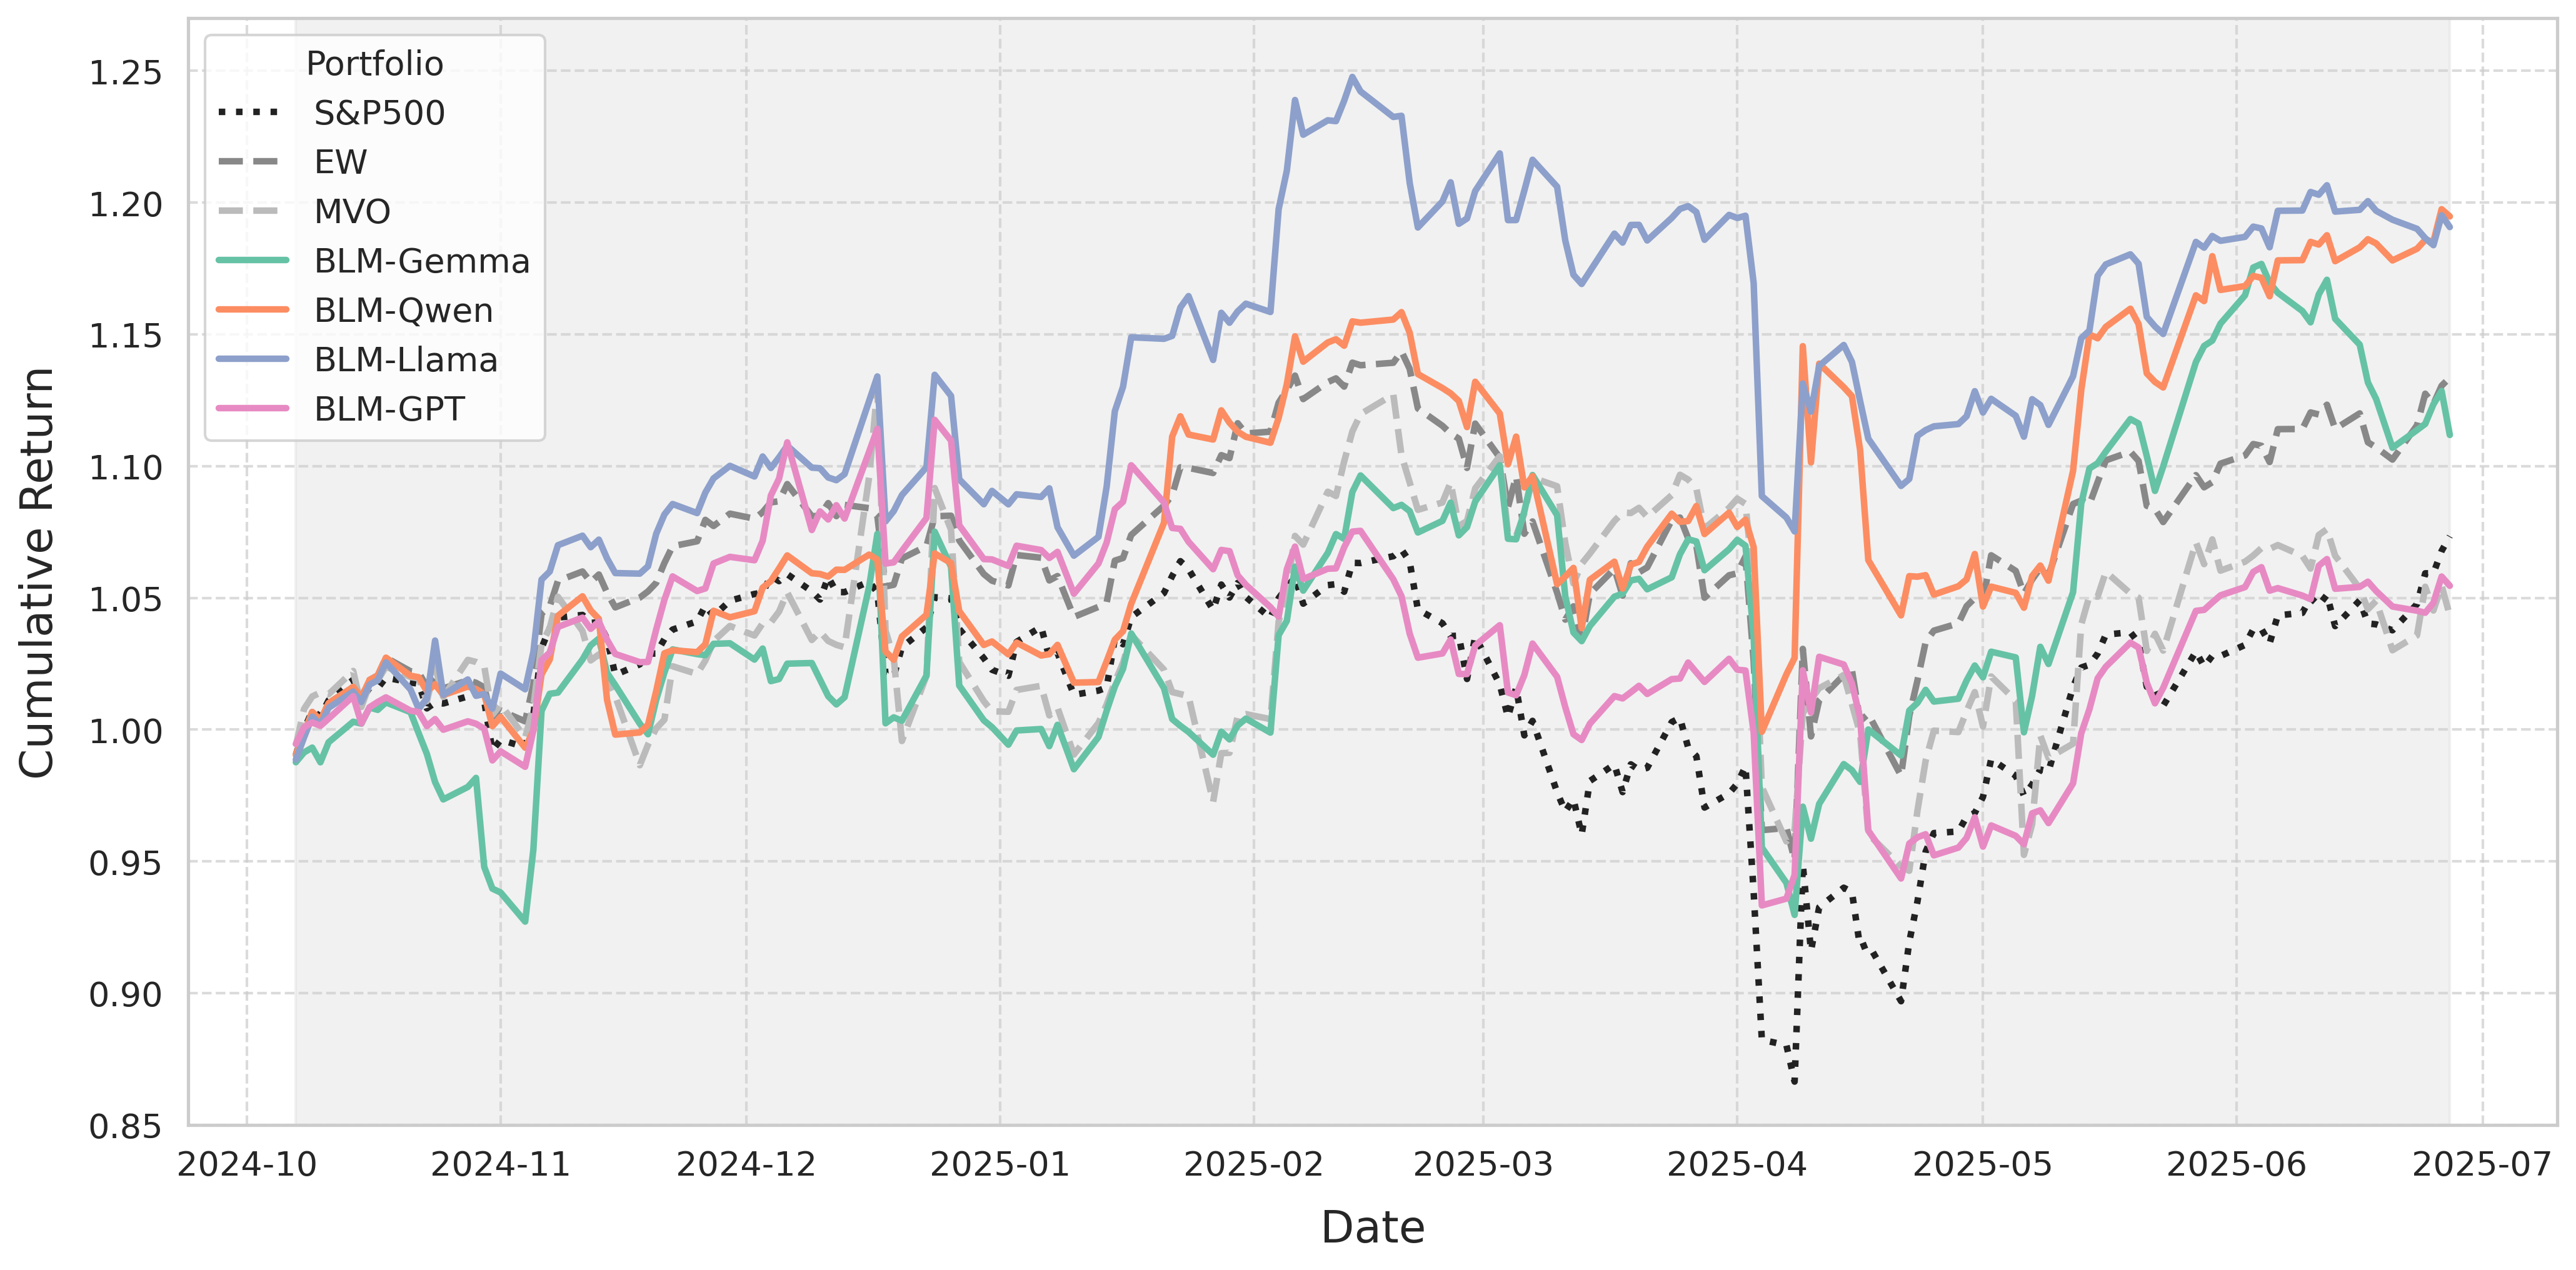
\includegraphics[width=0.9\textwidth]{figure/cumulative_returns_prompt4.png}  
    \caption{
    \textbf{Comparative Analysis of Cumulative Returns for BLM and Benchmark Portfolios.} The results highlight the significant outperformance of the \textbf{\texttt{BLM-Qwen}} and \textbf{\texttt{BLM-Llama}} strategies, which consistently generated higher returns compared to both the market index and conventional quantitative models.}
    \label{fig:cumulative_returns}  
\end{figure}
Conversely, the underperformance of \textbf{\texttt{BLM-Gemma}} and \textbf{\texttt{BLM-GPT}} corresponds to their higher prediction errors. High regression errors and lower classification accuracy in these models likely introduced noise into the posterior estimates, degrading the efficiency of the optimized portfolios.


% \begin{table}[h!]
%     \centering
%     \caption{\textbf{Comparison of Prediction Errors and Classification Metrics}}
%     \label{tab:prediction_metrics}
%     \renewcommand{\arraystretch}{1.2}
%     % siunitx 설정: 숫자를 소수점 4자리로 정렬
%     \sisetup{
%         round-mode=places,
%         round-precision=4,
%         detect-weight=true,
%         table-format=1.4 % 정수 1자리, 소수 4자리
%     }
%     \small
%     \setlength{\tabcolsep}{5pt}
%     % tabularx 대신 tabular와 siunitx의 S column을 사용
%     \begin{tabular}{l S S S S S}
%     \toprule
%     \textbf{Metric} & {\textbf{MVO}} & {\textbf{\texttt{BLM-Gemma}}} & {\textbf{\texttt{BLM-Qwen}}} & {\textbf{\texttt{BLM-Llama}}} & {\textbf{\texttt{BLM-GPT}}} \\
%     \midrule
%     CAGR \(\uparrow\) & 0.0607 & 0.1590 & \bfseries 0.2811 & \ul{0.2751} & 0.0768 \\
%     Sharpe \(\uparrow\) & 0.0176 & 0.0402 & \ul{0.0669} & \bfseries 0.0774 & 0.0228 \\
%     \midrule
%     MSE $\downarrow$  & 0.9376 & 1.2373 & \bfseries 0.5125 & \ul{0.5288} & 0.6505 \\
%     RMSE $\downarrow$ & 0.9683 & 1.1123 & \bfseries 0.7159 & \ul{0.7272} & 0.8066 \\
%     MAE $\downarrow$  & 0.6989 & 0.8608 & \bfseries 0.5168 & \ul{0.5281} & 0.5702 \\
%     \midrule
%     Accuracy $\uparrow$  & {0.5059} & 0.4719 & \bfseries 0.5719 & \ul{0.5437} & 0.5215 \\
%     Precision $\uparrow$ & {0.5689} & 0.5648 & \bfseries 0.5781 & \ul{0.5689} & 0.5645 \\
%     Recall $\uparrow$    & {0.5711} & 0.3437 & \bfseries 0.9367 & \ul{0.8424} & 0.7235 \\
%     F1 $\uparrow$        & {0.5700} & 0.4273 & \bfseries 0.7150 & \ul{0.6792} & 0.6342 \\
%     \bottomrule
%     \end{tabular}
% \end{table}


\begin{table}[h!]
    \centering
    \caption{\textbf{Comparison of Portfolio and Predictive Performance Metrics}}
    \label{tab:prediction_metrics}
    \renewcommand{\arraystretch}{1.2}
    
    % siunitx 설정
    \sisetup{
        round-mode=places,
        round-precision=4,
        detect-weight=true,
        table-format=1.4
    }
    \small
    \setlength{\tabcolsep}{4pt} % 컬럼이 늘어났으므로 간격을 조금 좁힘
    
    % 컬럼 정의: 맨 앞에 그룹용 'l' 추가 (총 7개 컬럼)
    \begin{tabular}{l l S S S S S}
    \toprule
    & \textbf{Metric} & {\textbf{MVO}} & {\textbf{\texttt{BLM-Gemma}}} & {\textbf{\texttt{BLM-Qwen}}} & {\textbf{\texttt{BLM-Llama}}} & {\textbf{\texttt{BLM-GPT}}} \\
    \midrule
    
    % --- Group 1: Portfolio Performance ---
    \multirow{2}{*}{\shortstack[l]{\textbf{Portfolio}\\\textbf{Performance}}} 
        & CAGR \(\uparrow\)    & 0.0607 & 0.1590 & \bfseries 0.2811 & \ul{0.2751} & 0.0768 \\
        & Sharpe \(\uparrow\)  & 0.0176 & 0.0402 & \ul{0.0669} & \bfseries 0.0774 & 0.0228 \\
    \midrule
    
    % --- Group 2: Regression ---
    \multirow{3}{*}{\shortstack[l]{\textbf{Predictive}\\\textbf{Performance}\\\textbf{(Regression)}}} 
        & MSE $\downarrow$     & 0.9376 & 1.2373 & \bfseries 0.5125 & \ul{0.5288} & 0.6505 \\
        & RMSE $\downarrow$    & 0.9683 & 1.1123 & \bfseries 0.7159 & \ul{0.7272} & 0.8066 \\
        & MAE $\downarrow$     & 0.6989 & 0.8608 & \bfseries 0.5168 & \ul{0.5281} & 0.5702 \\
    \midrule
    
    % --- Group 3: Classification ---
    \multirow{4}{*}{\shortstack[l]{\textbf{Predictive}\\\textbf{Performance}\\\textbf{(Classification)}}} 
        & Accuracy $\uparrow$  & {0.5059} & 0.4719 & \bfseries 0.5719 & \ul{0.5437} & 0.5215 \\
        & Precision $\uparrow$ & {0.5689} & 0.5648 & \bfseries 0.5781 & \ul{0.5689} & 0.5645 \\
        & Recall $\uparrow$    & {0.5711} & 0.3437 & \bfseries 0.9367 & \ul{0.8424} & 0.7235 \\
        & F1 $\uparrow$        & {0.5700} & 0.4273 & \bfseries 0.7150 & \ul{0.6792} & 0.6342 \\
    \bottomrule
    \end{tabular}
\end{table}
 % \label{tab:prediction_errors}



\subsection{RQ2: Investment Styles - View}

To further investigate the characteristics of the formulated asset views, we analyzed the distribution of their values. Figure~\ref{fig:boxplot} displays a time-series of these distributions. Since a single view corresponds to a specific asset, each boxplot on the chart represents the cross-sectional distribution of views across the $n$ assets for that rebalancing period. This visualization reveals how the dispersion of the model's expected returns evolves over time. The y-axis is clipped to a range of -0.03 to 0.03 for clarity, and the summary statistics in Table~\ref{tab:view_statistics} provide details on the aggregate distribution across all periods.

\begin{figure}[H]
    \centering
    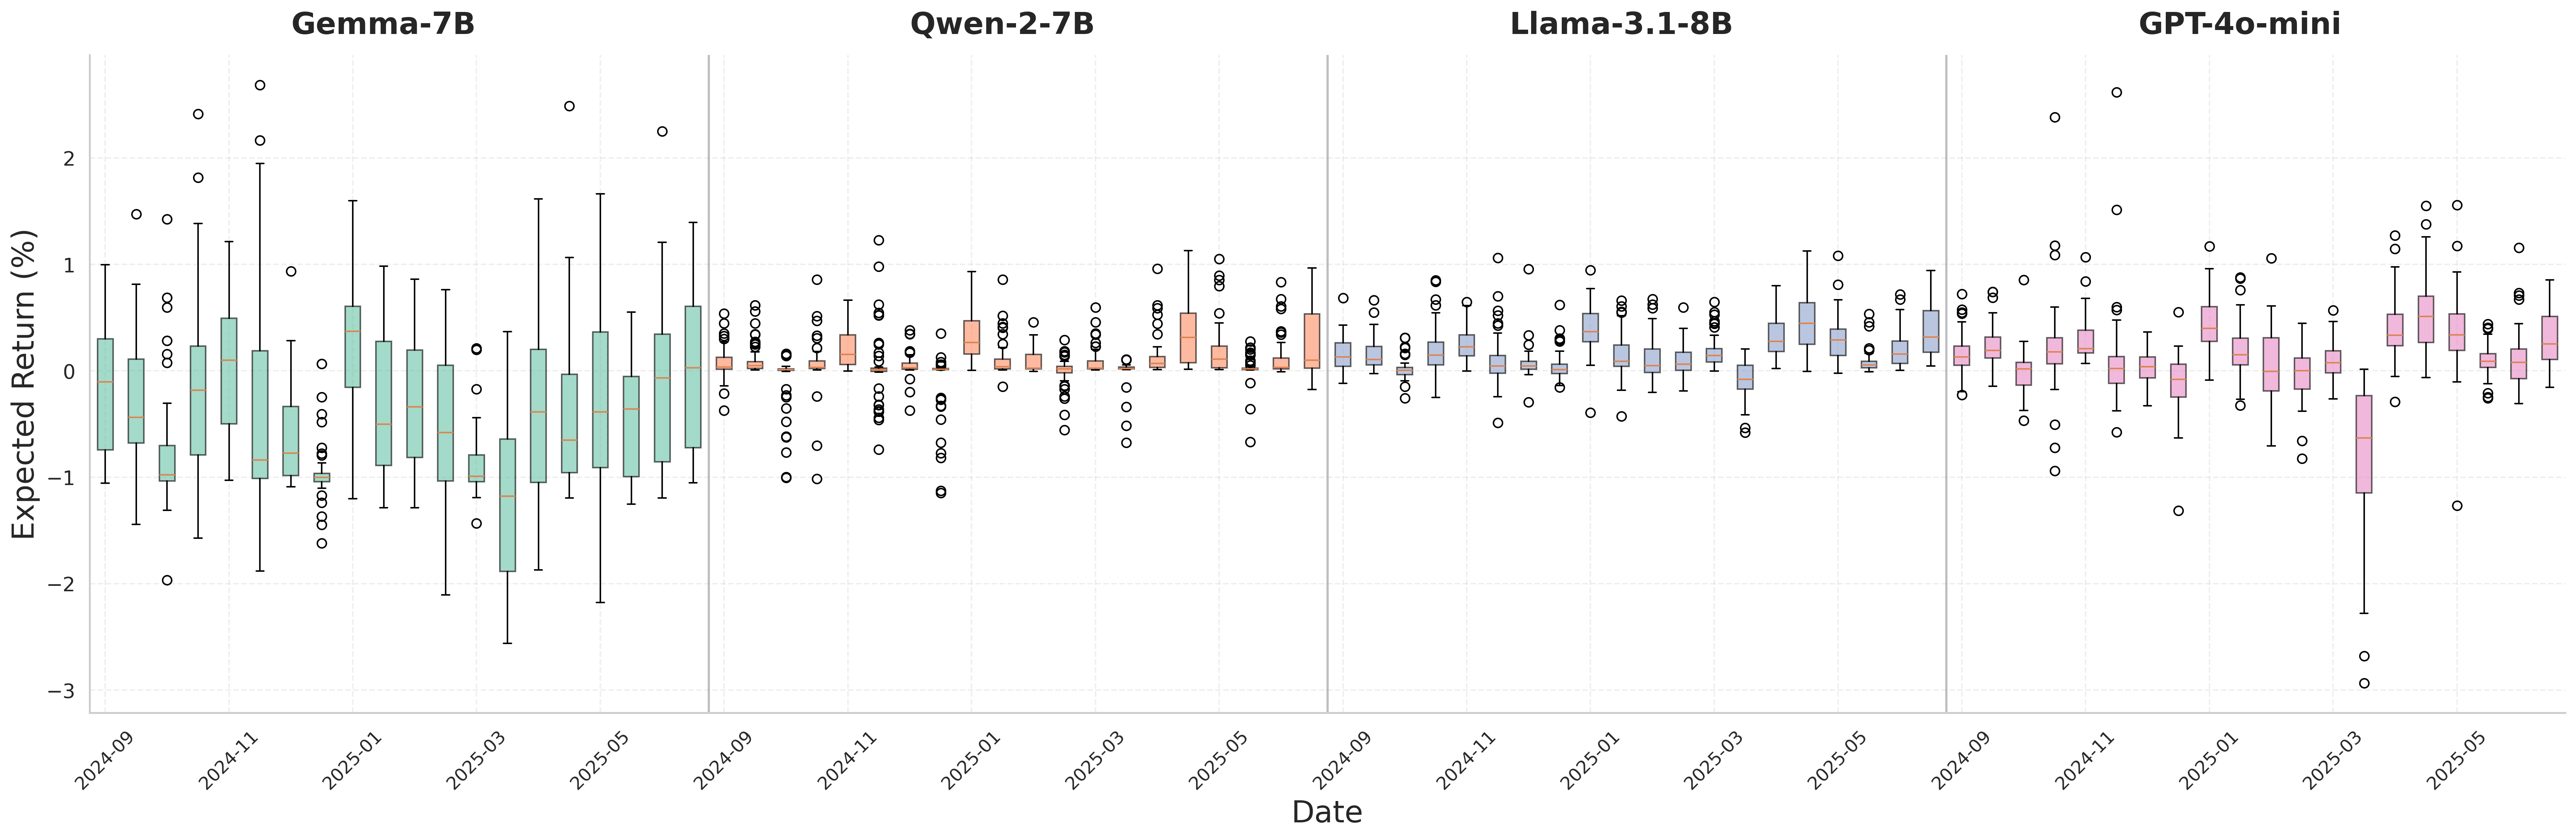
\includegraphics[width=1.0\textwidth]{figure/views_boxplot_4.png} 
    \caption{
    \textbf{LLM-generated Views Over Time at Rebalancing Intervals.} The figure visualizes the distribution of all generated return forecasts for each LLM at every rebalancing interval. 
    }
    \label{fig:boxplot} 
\end{figure}

The visual analysis highlights observable differences in the distributional patterns of each model's forecasts. These differences are consistent with recent findings that LLMs are not neutral decision-makers but possess distinct, model-specific biases \cite{lee2025your}. 
\textbf{\texttt{Gemma}} shows a relatively wider interquartile range compared to other models, indicating a higher degree of dispersion in its predicted returns. Additionally, its median values frequently sit slightly below zero, suggesting a tendency toward more conservative or negative return forecasts during the sample period.

In comparison, \textbf{\texttt{Qwen}} and \textbf{\texttt{Llama}} exhibit more concentrated distributions. Both models tend to produce forecasts clustered slightly above zero, with narrower interquartile ranges than \textbf{\texttt{Gemma}}. \textbf{\texttt{Qwen}} displays a tight core distribution while maintaining some distinct negative outliers, whereas \textbf{\texttt{Llama}} shows a similarly compact distribution. This suggests that, for this specific dataset, these models tended to generate lower-variance forecasts with a slightly positive central tendency.

Finally, \textbf{\texttt{GPT}} demonstrates variability in its dispersion over time. While often similar to the concentrated profiles of \textbf{\texttt{Qwen}} and \textbf{\texttt{Llama}}, it shows periods of increased variance, such as around March 2025, where the distribution widens and extends into negative territory.

Overall, these results indicate that even when prompted with the same instructions, different LLMs yield varying distributions of expected returns. \textbf{\texttt{Qwen}} and \textbf{\texttt{Llama}} provided more stable and slightly positive signals compared to the wider dispersion observed in \textbf{\texttt{Gemma}}. These distributional characteristics—specifically the lower variance and positive drift—likely contributed to the differences in portfolio allocation and subsequent performance discussed in the previous section.

Table~\ref{tab:view_statistics} provides the summary statistics for the entire population of raw views generated by each LLM throughout the test period. These statistics further illustrate the distributional differences suggested by the preceding visual analysis. For instance, \textbf{\texttt{Llama}} exhibits the highest mean return together with the largest standard deviation and the widest min-max range. In contrast, \textbf{\texttt{Qwen}} has the lowest standard deviation, while \textbf{\texttt{Gemma}} shows a negative mean during the sample period. Taken together, these summary statistics are broadly consistent with the differences in center and dispersion discussed above and may help explain the differences in portfolio behavior and performance.

\begin{table}[h!]
    \centering
    \caption{Summary Statistics of LLM-Generated Views}
    \label{tab:view_statistics}
    \renewcommand{\arraystretch}{1.2}
    % siunitx 설정: 숫자를 소수점 4자리로 정렬
    \sisetup{
        round-mode=places,
        round-precision=4,
        table-format=-2.4 % 부호, 정수 2자리, 소수 4자리
    }
    \small
    \setlength{\tabcolsep}{5pt}
    \begin{tabular}{l S S S S}
    \toprule
    \textbf{Metric} & {\textbf{\texttt{Gemma-7B}}} & {\textbf{\texttt{Qwen-2-7B}}} & {\textbf{\texttt{Llama-3.1-8B}}} & {\textbf{\texttt{GPT-4o-mini}}} \\
    \midrule
    \textbf{Count}      & \multicolumn{1}{c}{1000} & \multicolumn{1}{c}{1000} & \multicolumn{1}{c}{1000} & \multicolumn{1}{c}{1000} \\
    \textbf{Mean}       & -0.3847       & 0.1007        & 0.1786        & 0.1347        \\
    \textbf{Std}        & 0.7492        & 0.2430        & 0.2248        & 0.4171        \\
    \textbf{Min}        & -2.5617       & -1.1486       & -0.5812       & -2.9331       \\
    \textbf{25\%}       & -0.9917       & 0.0159        & 0.0290        & -0.0299       \\
    \textbf{Median}     & -0.5152       & 0.0343        & 0.1169        & 0.1295        \\
    \textbf{75\%}       & 0.1607        & 0.1519        & 0.2923        & 0.3191        \\
    \textbf{Max}        & 2.6854        & 1.2284        & 1.1264        & 2.6172        \\
    \bottomrule
    \end{tabular}
\par\small\textit{Note:} All metrics except `Count' are expressed in percentages (\%).
\end{table} % \label{tab:view_statistics}

\subsection{RQ3: Investment Styles - Confidence}

Finally, we investigate the association between the model-implied confidence and the realized prediction error. In the BLM framework, this relationship is relevant because the confidence matrix $\Omega$ acts as a weighting mechanism: views with higher volatility are effectively down-weighted during the posterior update. Figure~\ref{fig:scatter} plots the correlation between view standard deviation (x-axis) and RMSE (y-axis) for each model, superimposed with linear regression lines.

\begin{wrapfigure}{r}{0.5\textwidth}
    \centering
    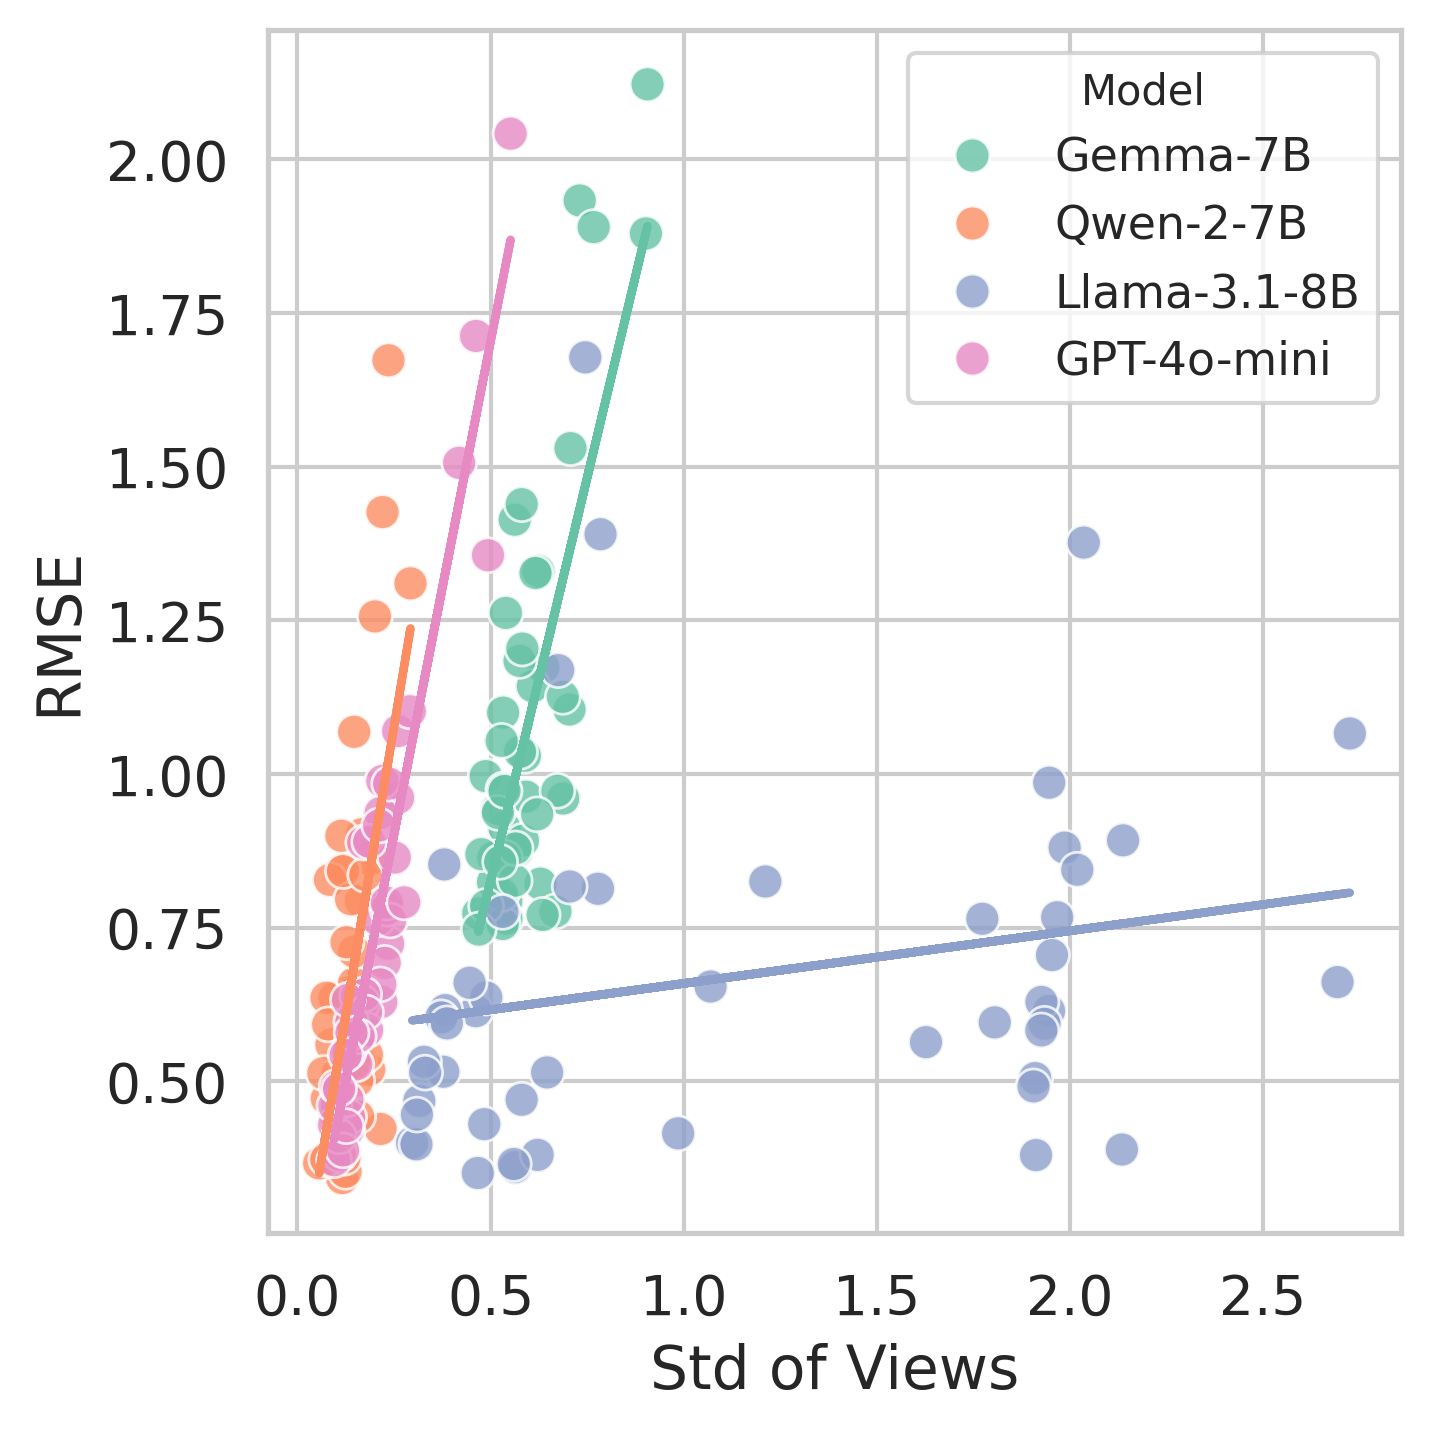
\includegraphics[width=\linewidth]{figure/scatter_4_scaled-none.png}
    \caption{\textbf{Correlation between view standard deviation and prediction error.}   }
    \label{fig:scatter}
    \vspace{-10pt} 
\end{wrapfigure}

\textbf{\texttt{Llama}} exhibits a relatively flat trajectory. The regression line has a near-zero slope ($0.086$) positioned at the lowest RMSE level among the tested models. This indicates that, in our experiment, \textbf{\texttt{Llama}}'s prediction error remained consistently low regardless of the magnitude of its estimated variance. This suggests that the model's contribution to the portfolio was driven primarily by its lower baseline error rather than the variance-based filtering mechanism.

In contrast, \textbf{\texttt{Qwen}} demonstrates the steepest positive slope ($3.751$). This positive correlation implies that instances where the model reported lower variance (higher confidence) tended to correspond with lower prediction errors. Within the BLM framework, this alignment allows the optimizer to effectively down-weight predictions that are likely to have high variance (low confidence), potentially aiding portfolio stability. This observation shares similarities with the findings in \cite{lee2025return}, which highlighted that portfolio performance is often driven by accurate predictions specifically for the assets selected in the portfolio, rather than global accuracy. 

Conversely, \textbf{\texttt{Gemma}} (slope: $2.621$) and \textbf{\texttt{GPT}} (slope: $3.204$) show distributions clustered in regions of higher overall RMSE compared to \textbf{\texttt{Llama}} and \textbf{\texttt{Qwen}}. 
While they also display positive slopes, indicating some correspondence between uncertainty and error, their generally higher prediction errors suggest that the variance filter alone was insufficient to fully mitigate the impact of inaccurate views in this specific setting.

In summary, we observe distinct patterns in how the models' uncertainty estimates relate to their accuracy. \textbf{\texttt{Llama}} is characterized by a consistently lower error profile, whereas \textbf{\texttt{Qwen}} shows a stronger alignment between uncertainty and error magnitude. These results suggest that the efficacy of LLM-based views in a Bayesian framework may depend on either maintaining a low baseline error or successfully calibrating uncertainty estimates to realized risk.
\section{Conclusion}

We propose an auditable mapping from stochastic LLM forecasts to Black–Litterman views, treating the mean of stochastic forecasts as investor views and their predictive dispersion as confidence levels. To validate this protocol, we conducted an out-of-sample backtest over a 10-month period using large-cap equities. The results demonstrated that portfolios driven by signals from a subset of the tested models demonstrated the potential to enhance portfolio performance compared to both equal‑weight and mean-variance benchmarks after transaction costs. 

While our primary contribution is establishing this robust protocol, the experiments yielded preliminary observations regarding model behavior.
Primarily, we observed that utilizing models with higher baseline forecasting accuracy appeared to support better portfolio performance.
Secondary observations regarding distributional patterns and uncertainty alignment suggest that the framework's effectiveness may also depend on model-specific characteristics, such as the generation of concentrated forecasts or the calibration of reported confidence.

We emphasize, however, that these observations are strictly conditional on our specific experimental design.
Crucially, the performance rankings are limited to the inference settings employed in this study; variations in prompt engineering, sampling temperature, reasoning steps (e.g., Chain-of-Thought), or model versions could yield significantly different outcomes. 
Therefore, our results should be interpreted as a validation of the proposed framework's viability rather than a definitive evaluation of any specific model's financial capability.
% Future research could extend this work by estimating joint views across assets, incorporating timestamped financial text under strict information sets, or exploring regime‑aware model selection over longer investment horizons.

% \bibliographystyle{elsarticle-num} 
\bibliographystyle{elsarticle-harv} % EAAI (Examples: "as demonstrated (Allan, 2020a, 2020b; Allan and Jones, 2019)" or "as demonstrated (Jones, 2019; Allan, 2020). Kramer et al. (2023) have recently shown".)
\bibliography{EAAI}

\newpage

%\section*{Acknowledgment}
%This work was supported by the National Research Foundation of Korea (NRF) grant funded by the Korea government (MSIT) (No. RS-2025-24803208) and the Institute of Information \& Communications Technology Planning \& Evaluation (IITP) grant funded by the Korea government (MSIT) (No. RS-2020-II201336, Artificial Intelligence Graduate School Program (UNIST)). This work was supported by a New Faculty Research Grant of Pusan National University, 2025.

\section*{Declaration of generative AI and AI-assisted technologies in the manuscript preparation process}
During the preparation of this work the author(s) used Gemini 2.5 Pro in order to refine the grammar and tone of the written text. Importantly, the research results, including the development of the code and the core scientific contributions, were carried out entirely without the assistance of LLMs. After using this tool/service, the author(s) reviewed and edited the content as needed and take(s) full responsibility for the content of the published article.

\end{document}

